%!TEX root = pag0.tex
\chapter{Esperimenti}
\label{chapter5}
Nel capitolo ~\ref{chapter4} abbiamo parlato di due metodi per stimare il fattore di scala. Il primo è un metodo semplificato, dove la stima è fatta solo su di un campione e non c'è modo di verificare se questo valore è corretto. Se questa stima sbaglia, l'errore che genera viene portato avanti fino alla fine dell'esperimento. Come si vede in figura ~\ref{fig:1_metodo1} e ~\ref{fig:1_metodo2} la stima della scala con questo metodo, porti ad un errore massimo di stima della posizione di 1 cm per ogni spostamento effettuato.
\begin{figure}[H]
   \centering
   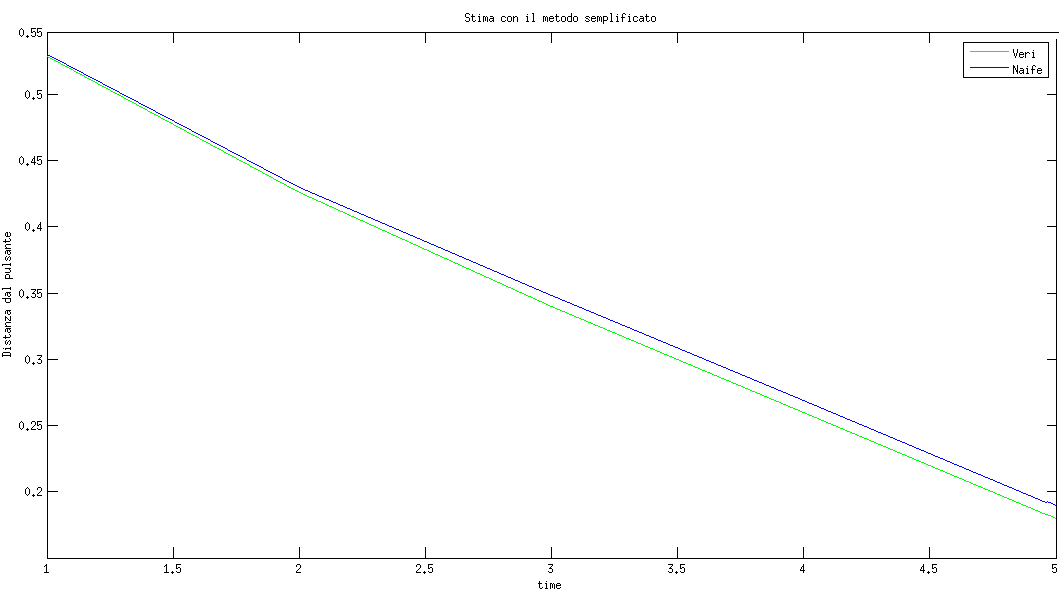
\includegraphics[width=1.\columnwidth]{naif25.png}
   \caption{Grafico dell'errore di stima della posa. In blu i dati stimati mentre in verde quelli reali}
   \label{fig:1_metodo1} 
\end{figure} 
\begin{figure}[H]
   \centering
   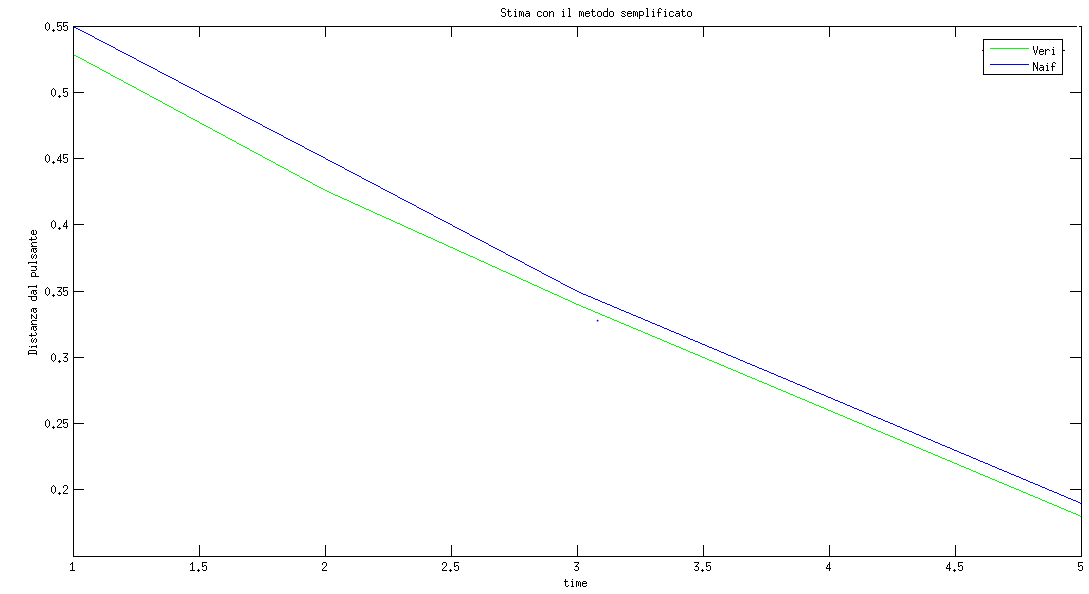
\includegraphics[width=1.\columnwidth]{naif28.png}
   \caption{Grafico dell'errore di stima della posa. In blu i dati stimati mentre in verde quelli reali}
   \label{fig:1_metodo2} 
\end{figure} 


Nel secondo metodo proposto invece, con l'utilizzo dello stimatore a massima verosomiglianza è possibile, utilizzando molti campioni, riuscire a far convergere l'errore di stima del fattore di scala al volore reale.
Per questo metodo occorro molti campioni. Per verificare la validità del metodo prendiamo un numero di campioni sufficientemente grande (maggiore di 500) di uno o più spostamenti. 
Per gli esperimenti si è scelto di utilizzare 1000 campioni di un unico spostamento, la convergenza è raggiunta se la differenza tra due campioni successivi è minore di 0.0001.
Nelle figure ~\ref{fig:mxli1} e ~\ref{fig:mxli2} possiamo vedere la convergenza della stima della scala per due esperimenti effettuati.
\begin{figure}[H]
   \centering
   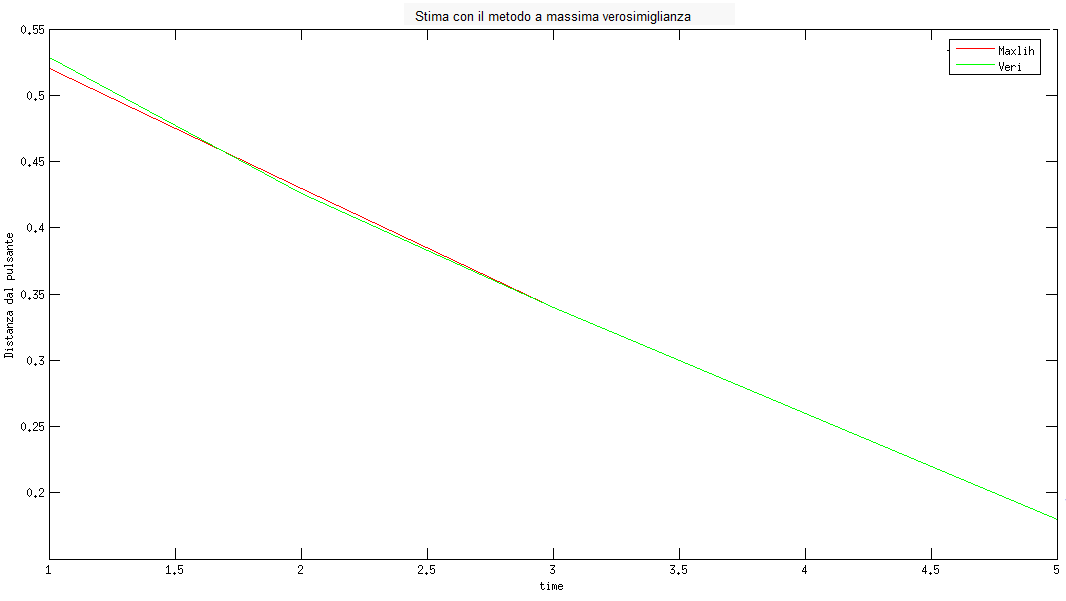
\includegraphics[width=1.\columnwidth]{maxlih24.png}
   \caption{Grafico dell'errore di stima della posa. In rosso i dati stimati mentre in verde quelli reali}
   \label{fig:mxli1} 
\end{figure} 
\begin{figure}[H]
   \centering
   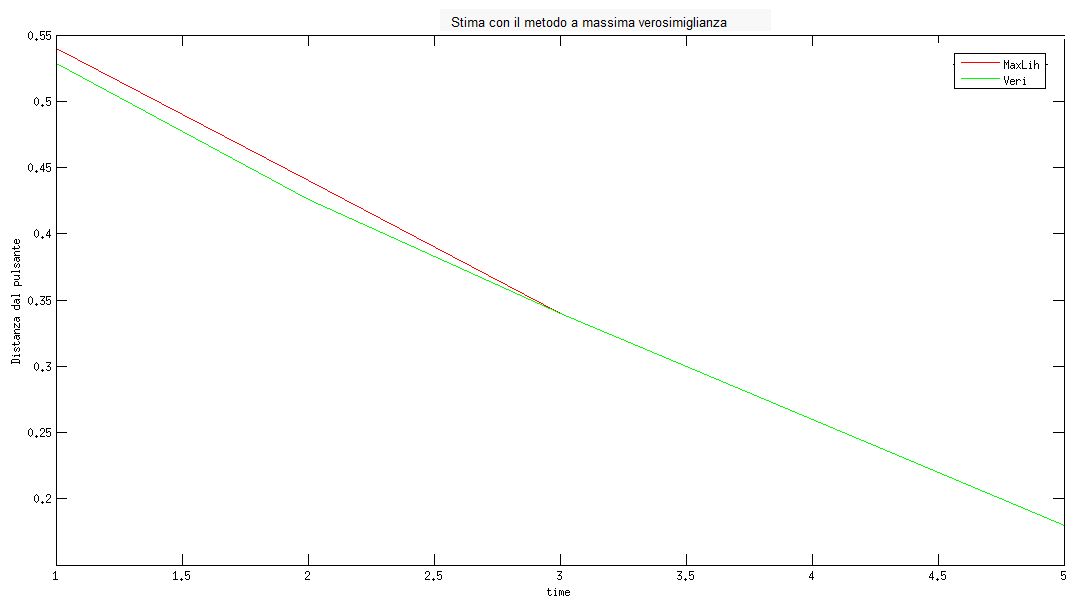
\includegraphics[width=1.\columnwidth]{maxlih28.png}
   \caption{Grafico della stima del valore di scala. In rosso i dati stimati mentre in verde quelli reali}
   \label{fig:mxli2} 
\end{figure} 
Nei due grafici sopra esposti si può vedere come la stima della scala con questo metodo, porti ad un errore massimo di qualche mm. 





\subsection{Confronto}
In figura  ~\ref{fig:confronto} mostriamo i confronti tra i due metodi per diversi set di dati.
\begin{figure*}
  \centering
  \subfigure[$confronto\_set1$]{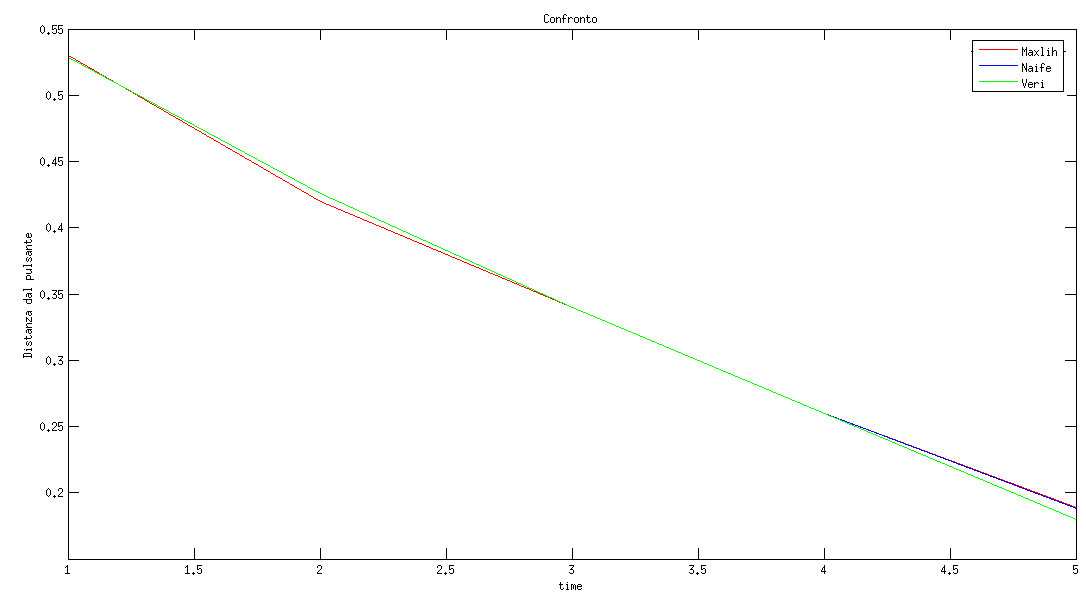
\includegraphics[width=1.\hsize]{Confrontoset24}\label{fig:confronto24}}
  \subfigure[$confronto\_set2$]{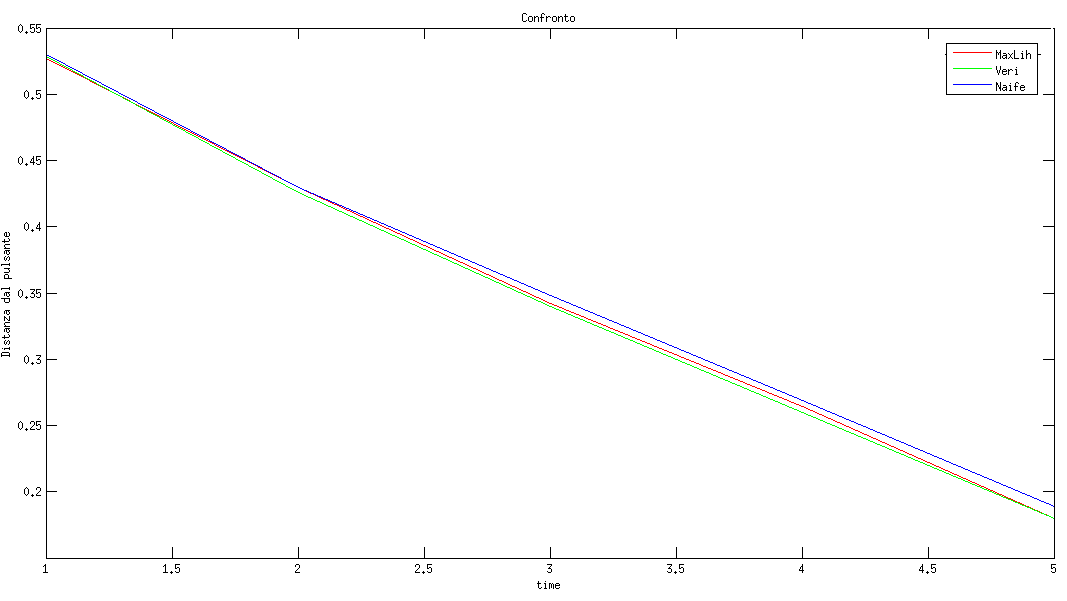
\includegraphics[width=1.\hsize]{Confrontoset25}\label{fig:confronto25}}
  % \subfigure[$confronto\_set3$]{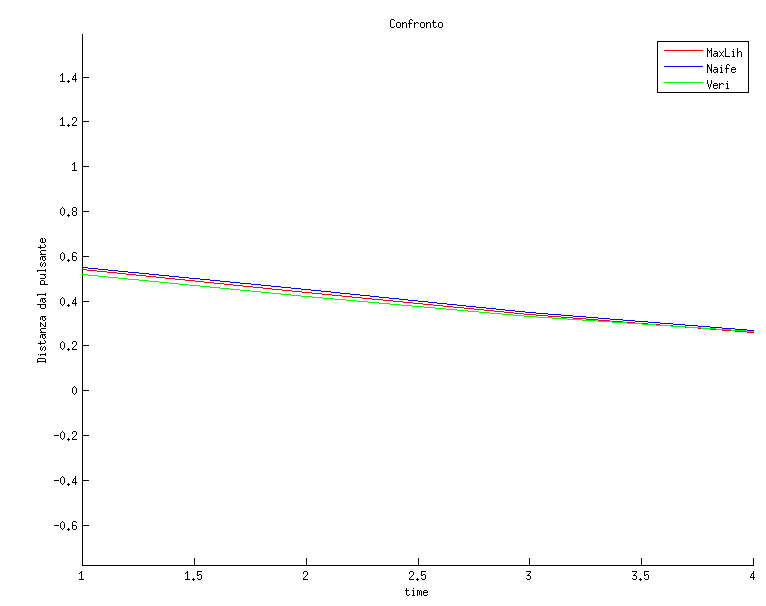
\includegraphics[width=1.\hsize]{Confronto28_1}\label{fig:confronto28}}
  \caption{Confronto tra i due metodi con la distanza effettiva}
  \label{fig:confronto}
\end{figure*}
Come possiamo vedere in figura ~\ref{fig:confronto} il metodo della massima verosimiglianza riesce a stimare meglio, nel lungo periodo, la posizione corretta della camera ottenendo un errore pari a 0.003 m. 
